% This is LLNCS.DOC the documentation file of
% the LaTeX2e class from Springer-Verlag
% for Lecture Notes in Computer Science, version 2.4
\documentclass[sigconf]{acmart}
%
\usepackage{graphicx}
\def\baselinestretch{0.96}
%\usepackage[pageanchor=true,hidelinks]{hyperref}
\usepackage{color}
\definecolor{mygray}{rgb}{0.6,0.6,0.6}
\definecolor{lightgray}{rgb}{0.92,0.92,0.92}
\definecolor{darkgreen}{rgb}{0,0.7,0}
\usepackage[justification=centering]{caption}
\captionsetup[table]{skip=1pt}
\usepackage{wrapfig}

% Great package for spaces in commands
\usepackage{xspace}

% for footnotes in tables
\usepackage{tablefootnote}

% for title caps
\usepackage{titlecaps}
\Addlcwords{and, the, or, of, that, our, by, a, prevent, for}
% We dont need page numbers according to https://www.sigapp.org/sac/sac2018/authorkit/author-kit-2018.pdf
\settopmatter{printacmref=false, printccs=true, printfolios=false}


% default options for listings
\usepackage{listings}
\usepackage{listingsutf8}
\usepackage{textcomp}     % access \textquotesingle
\lstset{
	backgroundcolor=\color{lightgray},
	basicstyle=\small\ttfamily\lst@ifdisplaystyle\scriptsize\fi,
	breaklines=true, 
	captionpos=b,
	commentstyle=\color{darkgreen}, 
	frame=single,
	keywordstyle=\color{blue}, 
	numbers=left,
	numbersep=5pt,
	numberstyle=\tiny\color{mygray},
	rulecolor=\color{black},
	showstringspaces=false,
	upquote=true,
	belowskip=-6ex,
}


\newcommand{\dq}[1]{``{#1}''}
%% THIS IS THE DATA FOR OUR THESIS, UPDATING HERE WILL UPDATE EVERYWHERE %%
\newcommand{\urls}{23,553,796\xspace}

\newcommand{\forms}{7,354,425\xspace}
\newcommand{\formsDelta}{31.22\%\xspace}

\newcommand{\emailforms}{1,228,774\xspace}
\newcommand{\emailformsDelta}{16.71\%\xspace}

\newcommand{\fuzzed}{1,012,530\xspace}
\newcommand{\fuzzedDelta}{82.40\%\xspace}

\newcommand{\recd}{74,192\xspace}
\newcommand{\recdDelta}{7.33\%\xspace}

\newcommand{\diffFoundFuzz}{9,682\xspace}
\newcommand{\malfuzzed}{64,510\xspace}
\newcommand{\malfuzzedDelta}{86.95\%\xspace}

\newcommand{\success}{994\xspace}
\newcommand{\successDelta}{1.54\%\xspace}
\newcommand{\successWebsitesDelta}{0.038\%\xspace} % calc domains/total_domains 414/1,085,365

\newcommand{\slowSelenium}{31.58\%\xspace}
\newcommand{\slowParse}{11.05\%\xspace}

\newcommand{\domains}{414\xspace}
\newcommand{\ips}{604\xspace}

\newcommand{\emailedDefaultmailbox}{113\xspace}
\newcommand{\responses}{21\xspace}
\newcommand{\confirmed}{15\xspace}


\newcommand{\ipsblacklist}{157\xspace}
\newcommand{\ipsblacklistmulti}{46\xspace}

\newcommand{\ehibcc}{583\xspace}
\newcommand{\ehixcheck}{493\xspace}
\newcommand{\ehito}{229\xspace}
\newcommand{\ehibccxcheck}{310\xspace}
\newcommand{\ehitoxcheck}{15\xspace}
\newcommand{\ehinuserxcheck}{239\xspace}
\newcommand{\ehiuniquenuserxcheck}{182\xspace}

% these refer to unique domains, not unique forms
\newcommand{\uniqueforms}{1,085,365\xspace}
\newcommand{\uniqueemailforms}{198,306\xspace}

\newcommand{\totalattachmentcount}{2,950\xspace}
\newcommand{\totalvirusattachmentcount}{265\xspace}
\newcommand{\totalvirusemails}{443\xspace}

\newcommand{\ehi}{E-\nobreak{}mail header injection\xspace}
\newcommand{\emails}{\email{}s\xspace}
\newcommand{\emailed}{\email{}ed\xspace}    
\newcommand{\Email}{E-\nobreak{}mail\xspace}        
\newcommand{\Emails}{\Email{}s\xspace}

\widowpenalty=10000
\clubpenalty=10000


\begin{document}
% Adding this here as instructed in the ACM e-mail, even though it works fine outside too.
\copyrightyear{2018}
\acmYear{2018}
\setcopyright{acmcopyright}
\acmConference[SAC 2018]{SAC 2018: Symposium on Applied Computing }{April
	9--13, 2018}{Pau, France}
\acmBooktitle{SAC 2018: SAC 2018: Symposium on Applied Computing , April 9--13,
	2018, Pau, France}
\acmPrice{15.00}
\acmDOI{10.1145/3167132.3167308}
\acmISBN{978-1-4503-5191-1/18/04}
	
\title{Measuring E-Mail Header Injections on the World Wide Web}\titlenote{This work was partially supported by a grant from the Center for Cybersecurity and Digitial Forensics at Arizona State University}

\lineskiplimit=-100pt\relax
\author{Sai Prashanth Chandramouli$^\dag$, Pierre-Marie Bajan$^\ddag$, Christopher Kruegel$^\S$}
\author{Giovanni Vigna$^\S$, Ziming Zhao$^\dag$, Adam Doup\'e$^\dag$, and Gail-Joon Ahn$^\dag$$^\tau$}
\affiliation{%
  \institution{$^\dag$Arizona State University, $^\ddag$IRT SystemX, $^\S$University of California, Santa Barbara, $^\tau$Samsung Research\\
    $^\dag$\{saipc, zzhao30, doupe, ahn\}@asu.edu, $^\ddag$pierre-marie.bajan@irt-systemx.fr, $^\S$\{chris, vigna\}@cs.ucsb.edu
  }
}

%% \author{Sai Prashanth Chandramouli$^\dag$, Pierre-Marie Bajan, Christopher Kruegel$^\ddag$,
%%   Giovanni Vigna$^\ddag$, Ziming Zhao$^\dag$, Adam Doup\'e$^\dag$, Gail-Joon Ahn$^\dag$}
%% \affiliation{%
%%   \institution{$^\dag$Arizona State University}
%% }
%% \email{$^\ddag$\{saipc, zzhao30, doupe, ahn\}@asu.edu}

%% \author{Sai Prashanth Chandramouli}
%% \affiliation{%
%% 	\institution{Arizona State University}
%% }
%% \email{saipc@asu.edu}

%% \author{Pierre-Marie Bajan}
%% \affiliation{%
%% 	\institution{ IRT SystemX}
%% }
%% \email{pierre-marie.bajan@irt-systemx.fr}

%% \author{Christopher Kruegel}
%% \affiliation{%
%% 	\institution{University of California, Santa Barbara}
%% }
%% \email{chris@cs.ucsb.edu}

%% \author{Giovanni Vigna}
%% \affiliation{%
%% 	\institution{University of California, Santa Barbara}
%% }
%% \email{vigna@cs.ucsb.edu}

%% \author{Ziming Zhao}
%% \affiliation{%
%% 	\institution{Arizona State University}
%% }
%% \email{zzhao30@asu.edu}


%% \author{Adam Doup\'e}
%% \affiliation{%
%% 	\institution{Arizona State University}
%% }
%% \email{doupe@asu.edu}

%% \author{Gail-Joon Ahn}
%% \affiliation{%
%% 	\institution{Arizona State University}
%% }
%% \email{gahn@asu.edu}

\renewcommand{\shortauthors}{S. Chandramouli, P. Bajan, C. Kruegel, G. Vigna, Z. Zhao, A. Doup\'e, and G. Ahn}


\renewcommand{\email}{e-\nobreak{}mail\xspace}
\vspace{-2.5ex}
\begin{abstract}
	\ehi vulnerability is a class of vulnerability that can occur in
    web applications that use user input to construct \email messages.
    \ehi vulnerabilities exist in the built-in \email functionality of
    the popular languages PHP, Java, Python, and Ruby. With the proper
    injection string, this vulnerability can be exploited to allow an
    attacker to inject additional headers, modify existing headers,
    and alter the content of the \email.

	While \ehi vulnerabilities are known to the community, and some
    commercial vulnerability scanners claim to discover \ehi
    vulnerabilities, they have never been studied by the academic
    community. This paper presents a scalable mechanism to
    automatically detect \ehi vulnerabilities and uses this mechanism
    to quantify the prevalence of \ehi vulnerabilities on the web.
    From crawling \urls URLs, we found \success vulnerable URLs across
    \domains domains. 135 of these domains are in the Alexa top 1
    million, and five of them are in the top 20,000. 137 of the
    vulnerable domains are using anti-spoofing mechanisms such as
    DKIM, SPF, or DMARC, and \ehi renders this protection useless.
    This work shows that \ehi vulnerabilities are widespread and
    deserve future research attention.
\end{abstract}


\begin{CCSXML}
	<ccs2012>
	<concept>
	<concept_id>10002978.10003022</concept_id>
	<concept_desc>Security and privacy~Software and application security</concept_desc>
	<concept_significance>500</concept_significance>
	</concept>
	<concept>
	<concept_id>10002978.10003022.10003026</concept_id>
	<concept_desc>Security and privacy~Web application security</concept_desc>
	<concept_significance>500</concept_significance>
	</concept>
	</ccs2012>
\end{CCSXML}

\ccsdesc[500]{Security and privacy~Software and application security}
\ccsdesc[500]{Security and privacy~Web application security}


\keywords{E-mail header injection, Software Security}

\maketitle

\lineskiplimit=0pt

\section{Introduction}\label{sec:Introduction}

The World Wide Web has single-handedly brought about a change in the way we use computers. The ubiquitous nature of the web makes it possible for anyone to access information and services anywhere and on multiple devices such as phones, laptops, TVs, and cars. This access has ushered in an era of web applications which depend on user input.
While the rapid pace of development has improved the speed of
information dissemination, it comes at a cost. As users move more and
more of their personal and financial information to web applications,
attackers are responding by using web application vulnerabilities to steal lucrative data.

Many common and well-known web application vulnerabilities, such as SQL Injection and Cross-Site Scripting~\cite{OWASPT10}, are command injection vulnerabilities~\cite{commandinjection}, where malicious user input is used to alter the structure of a command (SQL query and JavaScript code respectively). Developers of web applications must use the correct sanitization routine in all paths from user input to a command. 

\ehi vulnerabilities are a lesser-known command injection vulnerability. We verified that this vulnerability exists in the implementation of the built-in \email functionality in the popular languages PHP, Java, Python, and Ruby. The format of \email messages is defined by the Simple Mail Transfer Protocol (SMTP)~\cite{rfc5322}. Each \email message is represented by a series of headers separated by newlines, followed by the body content (separated from the headers by two newlines). Some of these headers are mandatory (\lstinline{From}, \lstinline{To}, \lstinline{Date}), but the headers could also include other information such as the \lstinline{Subject}, \lstinline{BCC}, etc.

With the proper exploit injection string, \ehi vulnerabilities can be exploited by an attacker to inject additional headers, modify existing headers, or alter the contents of the \email---while still appearing to be from a legitimate source. \ehi exploits allow an attacker to perform \email spoofing, resulting in phishing attacks \emph{that are sent from the actual \email server}, and thus bypass \email spoofing technologies, such as DKIM~\cite{allman2007domainkeys}, SPF~\cite{schlitt2006sender}, and DMARC~\cite{kucherawy2015domain}.

While some command injection vulnerabilities have received extensive attention from the research community, \ehi vulnerabilities have received little focus. In fact, the Acunetix vulnerability scanner contains an AcuMonitor component which claims to detect \ehi vulnerabilities while scanning~\cite{acumonitor}. Unfortunately, as a commercial product, little is known about how AcuMonitor detects \ehi vulnerabilities. 

To shed light on this little-studied vulnerability class, we describe
\ehi vulnerabilities and measure \ehi vulnerabilities. To perform this
measurement, we crawled the web, extracted forms with \email fields,
and injected them with different payloads to infer the existence of an
\ehi vulnerability. We then automatically audited received \emails to
see if any of the injected data was present. This allowed us to
classify whether a particular URL was vulnerable to the attack. Our
automated system works in a black-box manner, without looking at the
web application's source code, and only analyzes the payloads in the
\emails.\\\\

In summary, we make the following contributions:
\begin{itemize}

\item We develop a black-box approach to detect \ehi vulnerabilities in a web application.

\item We develop an open-source system to crawl the web and automatically detect \ehi vulnerabilities.

\item We use our system to crawl \urls URLs, and we find \success URLs vulnerable to \ehi across \domains domains. 

\item We perform detailed analyses on the domains found to be vulnerable: finding their Alexa rankings, the technologies used in such vulnerable domains, presence of \email spoofing protection, presence of such domains on existing spam-lists, and the ability to send malicious attachments.

\end{itemize}


\section{Background}
\vspace{-2.5ex}
\ehi belongs to the class of command injection vulnerabilities. However, unlike its more popular siblings, SQL injection~\cite{sql1,sql0,sql2}, Cross-Site Scripting~\cite{Injection1,KleinAmit}, or HTTP Header Injection~\cite{sessionride}, relatively little research is available on \ehi vulnerabilities.

As with other command injection vulnerabilities, \ehi is caused by
improper or nonexistent sanitization of user input. If the program
constructs \emails from user input and fails to check for the presence
of \email headers, a malicious user can control the headers of this particular e-mail. \ehi vulnerabilities can be leveraged to enable malicious attacks, including, but not limited to, spoofing or phishing.

\subsection{History of \ehi}

\begin{lstlisting}[language=PHP,caption={PHP program with e-mail
      header injection vulnerability.},label={code:phpemi}, float]
$from = $_REQUEST['email'];
$subject = 'Hello XYZ';
$message = 'We need you to reset your password';
$to = 'xyz@example.com';
$retValue = mail($to, $subject, $message, "From: $from");
\end{lstlisting}



\begin{table}[tbp]
  \scriptsize
	\centering
	\begin{tabular}{|c|p{5.5cm}|c|}
		\hline
		\multicolumn{1}{|c|}{\textbf{CVE No.}} & 
		\multicolumn{1}{c|}{\textbf{Affected Software}} &
		\multicolumn{1}{c|}{\textbf{Year}}\\
		\hline
		{2002-1575} & {cgiemail} & {2004}\\
		\hline
		{2002-1771} & {FormMail 1.9} & {2005}\\
		\hline
		{2002-1917} & {Geeklog 1.35} & {2005}\\
		\hline
		{2005-0493} & {Biz Mail Form <=2.2} & {2005}\\
		\hline
		{2005-2854} & {thesitewizard.com} & {2005}\\
		\hline
		{2005-3883} & {PHP mb\_send\_mail} & {2005}\\
		\hline
		{2006-0631} & {Perl mailback.pl} & {2006}\\
		\hline
		{2006-0712} & {Squishdot 1.5.0} & {2006}\\
		\hline
		{2006-1225} & {Drupal 4.5.0-4.5.8 and 4.6.0-4.6.8} & {2006}\\
		\hline
		{2006-1305} & {Microsoft Outlook 2000, 2002-03} & {2006}\\
		\hline
		{2006-2159} & {Russcom Network} & {2006}\\
		\hline
		{2006-2943} & {CGI-RESCUE WebFORM 4.1} & {2006}\\
		\hline
		{2006-2944} & {CGI-RESCUE FORM2MAIL 1.21} & {2006}\\
		\hline
		{2006-3171} & {CS-Forum <=0.82} & {2006}\\
		\hline
		{2006-3473} & {Drupal Module <=1.8.2.2} & {2006}\\
		\hline
		{2006-4344} & {CGI-Rescue Mail} & {2006}\\
		\hline
		{2006-7020} & {phpwcms 1.2.5-DEV} & {2007}\\
		\hline
		{2006-7087} & {Dotdeb PHP} & {2007}\\
		\hline
		{2007-1718} & {PHP 4.0-4.4.6 and 5.0-5.2.1} & {2007}\\
		\hline
		{2007-1898} & {Jetbox CMS 2.1} & {2007}\\
		\hline
		{2007-1900} & {FILTER\_VALIDATE\_EMAIL PHP} & {2007}\\
		\hline
		{2007-2731} & {Jetbox CMS 2.1} & {2007}\\
		\hline
		{2008-2105} & {Bugzilla} & {2008}\\
		\hline
		{2009-1469} & {IceWarp} & {2009}\\
		\hline
		{2008-7281} & {OTRS - Open Ticket Request System} & {2011}\\
		\hline
		{2014-2957} & {Exim} & {2014}\\
		\hline
		{2015-8476} & {PHPMailer} & {2015}\\
		\hline
		{2016-4803} & {dotCMS} & {2016}\\
		\hline

	\end{tabular}
	\caption{History of software found in Common Vulnerabilities and
      Exposures database affected by e-mail header injection
      vulnerability}
	\label{tab:history}
	\vspace{-2ex}
\end{table}
We found the first \ehi description in a late 2004 article on
phpsecure.info~\cite{Tobozo} accredited to user \lstinline|tobozo|
describing how an \ehi vulnerability existed in the implementation of
the \texttt{mail()} function in PHP and how it can be exploited. More
recently, a blog post by Damon Kohler~\cite{DK} and an accompanying
wiki article~\cite{Injection} describe the attack vector and outline
few defense measures for \ehi vulnerabilities.


%% As this vulnerability was initially found in the \texttt{mail()} function of PHP, \ehi can be traced to as early as the beginning of the 2000's, present in the \texttt{mail()} implementation of PHP 4.0. 
An example of the vulnerable code written in PHP is shown in Listing~\ref{code:phpemi}. This code takes in user input from \texttt{\$\_REQUEST[\textquotesingle email\textquotesingle]}, and stores it in the variable \texttt{\$from}, which is later passed to the \texttt{mail()} function to construct and send the e-mail.





\begin{lstlisting}[language=HTML,caption={SMTP headers generated by a PHP mail
  script.},label={code:smtpheaders}, float]
Received: from mail.ourdomain.com ([62.121.130.29])
  by xyz.com (Postfix) with ESMTP id 5A08E52C0154
  for <abc@example.com>; Sun, 20 Mar 2016 13:56:58 -0700 (MST)
From: abc@example.com
To: xyz@example.com
Subject: Hello XYZ
CC: spc@example.com
Date: Sun, 20 Mar 2016 13:56:58 -0700(MST)

We need you to reset your password
\end{lstlisting}

\begin{sloppypar}


When this code is given the malicious input
\texttt{\lstinline{abc@example.com\\nCC:spc@example.com}} as the value
of the \texttt{\$\_REQUEST[\textquotesingle email\textquotesingle]},
it generates the equivalent SMTP Headers shown in
Listing~\ref{code:smtpheaders}. It can be seen that the \lstinline{CC}
(carbon copy) header that we injected appears as part of the resulting
SMTP message. This will make the e-mail get sent to the e-mail address
specified as part of the \lstinline{CC} as well.

%\begin{table}[tbp]
  \scriptsize
	\centering
	\begin{tabular}{|c|p{5.5cm}|c|}
		\hline
		\multicolumn{1}{|c|}{\textbf{CVE No.}} & 
		\multicolumn{1}{c|}{\textbf{Affected Software}} &
		\multicolumn{1}{c|}{\textbf{Year}}\\
		\hline
		{2002-1575} & {cgiemail} & {2004}\\
		\hline
		{2002-1771} & {FormMail 1.9} & {2005}\\
		\hline
		{2002-1917} & {Geeklog 1.35} & {2005}\\
		\hline
		{2005-0493} & {Biz Mail Form <=2.2} & {2005}\\
		\hline
		{2005-2854} & {thesitewizard.com} & {2005}\\
		\hline
		{2005-3883} & {PHP mb\_send\_mail} & {2005}\\
		\hline
		{2006-0631} & {Perl mailback.pl} & {2006}\\
		\hline
		{2006-0712} & {Squishdot 1.5.0} & {2006}\\
		\hline
		{2006-1225} & {Drupal 4.5.0-4.5.8 and 4.6.0-4.6.8} & {2006}\\
		\hline
		{2006-1305} & {Microsoft Outlook 2000, 2002-03} & {2006}\\
		\hline
		{2006-2159} & {Russcom Network} & {2006}\\
		\hline
		{2006-2943} & {CGI-RESCUE WebFORM 4.1} & {2006}\\
		\hline
		{2006-2944} & {CGI-RESCUE FORM2MAIL 1.21} & {2006}\\
		\hline
		{2006-3171} & {CS-Forum <=0.82} & {2006}\\
		\hline
		{2006-3473} & {Drupal Module <=1.8.2.2} & {2006}\\
		\hline
		{2006-4344} & {CGI-Rescue Mail} & {2006}\\
		\hline
		{2006-7020} & {phpwcms 1.2.5-DEV} & {2007}\\
		\hline
		{2006-7087} & {Dotdeb PHP} & {2007}\\
		\hline
		{2007-1718} & {PHP 4.0-4.4.6 and 5.0-5.2.1} & {2007}\\
		\hline
		{2007-1898} & {Jetbox CMS 2.1} & {2007}\\
		\hline
		{2007-1900} & {FILTER\_VALIDATE\_EMAIL PHP} & {2007}\\
		\hline
		{2007-2731} & {Jetbox CMS 2.1} & {2007}\\
		\hline
		{2008-2105} & {Bugzilla} & {2008}\\
		\hline
		{2009-1469} & {IceWarp} & {2009}\\
		\hline
		{2008-7281} & {OTRS - Open Ticket Request System} & {2011}\\
		\hline
		{2014-2957} & {Exim} & {2014}\\
		\hline
		{2015-8476} & {PHPMailer} & {2015}\\
		\hline
		{2016-4803} & {dotCMS} & {2016}\\
		\hline

	\end{tabular}
	\caption{History of software found in Common Vulnerabilities and
      Exposures database affected by e-mail header injection
      vulnerability}
	\label{tab:history}
	\vspace{-2ex}
\end{table}
\end{sloppypar}

%TODO Adam: added this para abt E-Mail Header Injection history from CVE

We gathered reported Common Vulnerabilities and Exposures
(CVE)~\cite{cve} to get an idea of the distribution of
reported \ehi vulnerabilities over time. From the 28 reports we found (Table~\ref*{tab:history}), it can be seen that even though many vulnerabilities were found in earlier years (2005-07), there have been recently discovered \ehi vulnerabilities which suggests that it is still a very real and relevant threat to modern web security.



\subsection{Languages Affected}

\label{languages}
\noindent{\textbf{PHP}} was the first language found vulnerable to \ehi in its implementation of the \lstinline{mail()} function at the time of release of PHP~4.0. According to w3techs~\cite{W3techs}, PHP is used by 81.9\% of all websites.

After 13 further iterations of PHP since the 4.0 release (the current
version is 7.1), the \texttt{mail()} function is yet to be fixed after
15 years. However, the PHP documentation~\cite{PHPDocs} specifies that the \texttt{mail()} function does not protect against \ehi.
A working code sample with the vulnerability is shown in  Listing~\ref{code:phpemi}.

\begin{sloppypar}
A bug was filed about an \ehi vulnerability in Python's implementation of the \texttt{email.header} library and the header parsing functions allowing newlines in early 2009, which was followed by a partial patch in 2011.
\end{sloppypar}

Unfortunately, the bug fix was only for the \lstinline{email.header} package, and not for other frequently used packages such as\- \lstinline{email.parser}, where both the classic \lstinline{Parser()} and the newer \lstinline{FeedParser()} contain \ehi vulnerabilities even in the latest versions: \lstinline{2.7.11} and \lstinline{3.5}. The bug fix was also not backported to older versions of Python.
There is no mention of the vulnerability in the Python documentation for either library. Contrary to PHP's behavior of overwriting existing headers, Python only recognizes the first occurrence of a header, and ignores duplicate headers.

Java has a bug report about \ehi filed against its \texttt{JavaMail} API. A detailed write-up by Alexandre Herzog~\cite{Herzog.2014} contains a proof-of-concept program that exploits the API to inject headers.

From our testing, Ruby's built-in \texttt{Net::SMTP} library also has the vulnerability (not documented on the library's homepage).



\subsection{Exploitation}
\label{exploitation}
Successful exploitation of an \ehi vulnerability depends on where
injection occurs in the SMTP message. The attacker cannot alter parts
of the SMTP message that precede the injection location, but the
attacker has complete control over everything that follows. However,
similar to other command injection vulnerabilities, the remaining
parts of the SMTP message will always be appended to the attacker's
injection, so the attacker must contend with this. By
exploiting an \ehi vulnerability, an attacker can control who receives
the message (and can include multiple \texttt{CC} and \texttt{BCC}
recipients), the body, and possibly the subject (depending on if the subject header occurs
before/after the injection point and the language used).

\begin{lstlisting}[language=HTML,caption={Exploiting the \ehi
      vulnerability in Listing~\ref{code:phpemi} to control the
      recipients, subject, and body of the SMTP message.},label={code:ehiexploit}, float]
Received: from mail.ourdomain.com ([62.121.130.29])
  by xyz.com (Postfix) with ESMTP id 5A08E52C0154
  for <abc@example.com>; Sun, 20 Mar 2016 13:56:58 -0700 (MST)
From: abc@example.com
CC: 1@example.com, 2@example.com, 3@example.com
Subject: My Subject
Content-Type: multipart/mixed; boundary=foobar;
--foobar
Content-Type: text/html

This is the attacker's body
--foobar
To: xyz@example.com
Subject: Hello XYZ
Date: Sun, 20 Mar 2016 13:56:58 -0700(MST)

We need you to reset your password
\end{lstlisting}

The main vector for exploiting \ehi vulnerabilities follows the
template of command injection vulnerability exploitation: first inject
the attacker's desired commands, then comment out the rest of the
message. In \ehi vulnerabilities, the attacker first includes all SMTP
headers she desires. These will typically be the \texttt{Subject}
header to control the subject of the \email\footnotemark, \texttt{CC}
or \texttt{BCC} headers to control the recipients of the \email.

\footnotetext{The SMTP protocol
specifies that there should only be one \texttt{Subject} header, so
the attacker may not be able to alter the subject if the header is
already defined. This behavior would be MUA-dependent.
}

To handle the extra content after the injection point, one technique
is to use a \texttt{Content-type} header to specify that the SMTP
message is a multi-part email and that the sections are separated by
an attacker-specified boundary. The boundary delineates different
parts of the message so that the attacker's body is the only valid
part of the message, and the attacker can choose a random value for
the boundary that is not present in the developer-controlled part of
the SMTP message.

Using this technique, the attacker can completely control the \email.
For instance, injecting the following attack payload:
\texttt{\lstinline{abc@example.com\\nCC:1@example.com, 2@example.com,
    3@example.com\\nSubject: My
    Subject\\nContent-Type:multipart/mixed;
    boundary=foobar;\\n--foobar\\nContent-Type: text/html
    \\n\\nThis is the attacker's body\\n--foobar}} into the \texttt{email} parameter
of the PHP program in Listing~\ref{code:phpemi} results in
the SMTP message shown in Listing~\ref{code:ehiexploit}.

By expanding on this technique, the attacker can include links in the
\email, or even attachments, by adding additional multipart messages
with different content types.

A shorter technique, in case the injection point is limited in input
size, is to use an HTML comment to ignore the developer-controlled
part of the SMTP message, using a payload such as:
\texttt{\lstinline{abc@example.com\\nCC:1@example.com, 2@example.com,
    3@example.com\\nSubject: My Subject\\n
    Content-Type: text/html\\n\\nThis is the attacker's body<!--}}. However, this
technique will only work if the developer-controlled part of the SMTP
message does not contain a closing HTML comment tag
\texttt{\lstinline{-->}}.


\subsection{Impact of \ehi}

The impact of an \ehi vulnerability can be far-reaching. According to
w3tech, PHP, Java, Python, and Ruby (combined) account for over
85\%\, of the server-side programming languages in
websites measured, and the default implementation of the \email functionality of these languages is vulnerable to \ehi. 



%% \begin{table}[!tb]
%% 	\centering
%% 	\begin{tabular}{|p{4cm}|p{4cm}|}
%% 		\hline
%% 		\multicolumn{1}{|c|}{\textbf{Server Side Language}} & \multicolumn{1}{c|}{\textbf{\% of Usage}}\\
%% 		\hline
%% 		PHP & 81.9\\
%% 		\hline
%% 		Java & 3.1\\
%% 		\hline
%% 		Ruby & 0.6\\
%% 		\hline
%% 		Python & 0.2\\
%% 		\hline
		
%% 	\end{tabular}
%% 	\caption[\titlecap{Language usage statistics}]{Language usage statistics compiled from w3techs~\cite{W3techs}.}
%% 	\label{tab:usage}
%% \end{table}

An \ehi vulnerability can be exploited to do potentially any of the
following:

\noindent \textbf{Phishing and Spoofing Attacks} 
    Phishing~\cite{phishing} (a variation of spoofing~\cite{spoofing_attack}) refers to an attack where the recipient of an \email is made to believe that the \email is  legitimate when it was really created by a malicious party. The \email usually redirects the victim to a malicious website, which then steals their credentials or infects their computer with malware (via a drive-by-download).  
    
    \ehi gives attackers the ability to inject arbitrary headers into an \email sent by a website \emph{and control the output of the \email}. This adds credibility to the generated \email, as it is sent from the website's mail server and users (and anti-spam defenses) are more likely to trust an e-mail that is received from the proper mail server. Therefore, attackers could leverage \ehi vulnerabilities to perform enhanced phishing attacks. 
	
\noindent\textbf{Spam Networks}
	Spam networks can use \ehi vulnerabilities to send a large amount of \email from servers that are trusted. By adding additional \texttt{cc} or \texttt{bcc} headers to the generated e-mail, attackers can easily choose the recipient of the spam email. 
	
	Due to the \email being from trusted domains, recipient \email clients and anti-spam systems might not flag them as spam. If they do flag them as spam, then that can lead to the website being blacklisted as a spam generator (which would cause a Denial of Service on the vulnerable web application). 
	
\noindent\textbf{Information Extraction}
	\Emails can contain sensitive data that is meant to be accessed only by the user. Due to an \ehi vulnerability, an attacker can add a \texttt{bcc} header, and the \email server will send a copy of the \email to the attacker, thereby exposing important information.
	User privacy can thus be compromised, and loss of private information can lead to other attacks.

    \noindent\textbf{Denial of Service}
    Denial of service attacks (DoS), can also be caused by exploiting an \ehi vulnerability to send excessive \emails resulting in overloading the mail server and cause crashes or instability. 

%It is evident that E-Mail Header Injection is a critical vulnerability that web applications must address.



\vspace{-2.5ex}
\section{System Design}
\vspace{-2.5ex}
To quantify the existence of \ehi vulnerabilities on the web at large, we developed a system to automatically detect \ehi vulnerabilities in a black-box manner. 
\subsection{Approach}
\vspace{-2ex}
\label{sys:appr}
We took a black-box approach to measure the prevalence of \ehi
vulnerability on the web. Black-box
testing~\cite{Beizer:1995:BTT:202699} is a way to examine the
functionality of an application without analyzing its source code. Black-box testing allows our system to detect \ehi vulnerabilities in \emph{any} server-side language (not simply those we identified in Section~\ref{languages}). The overall architecture of our system is presented in Figure~\ref{fig:overall}. 

\begin{figure}
	\centering
	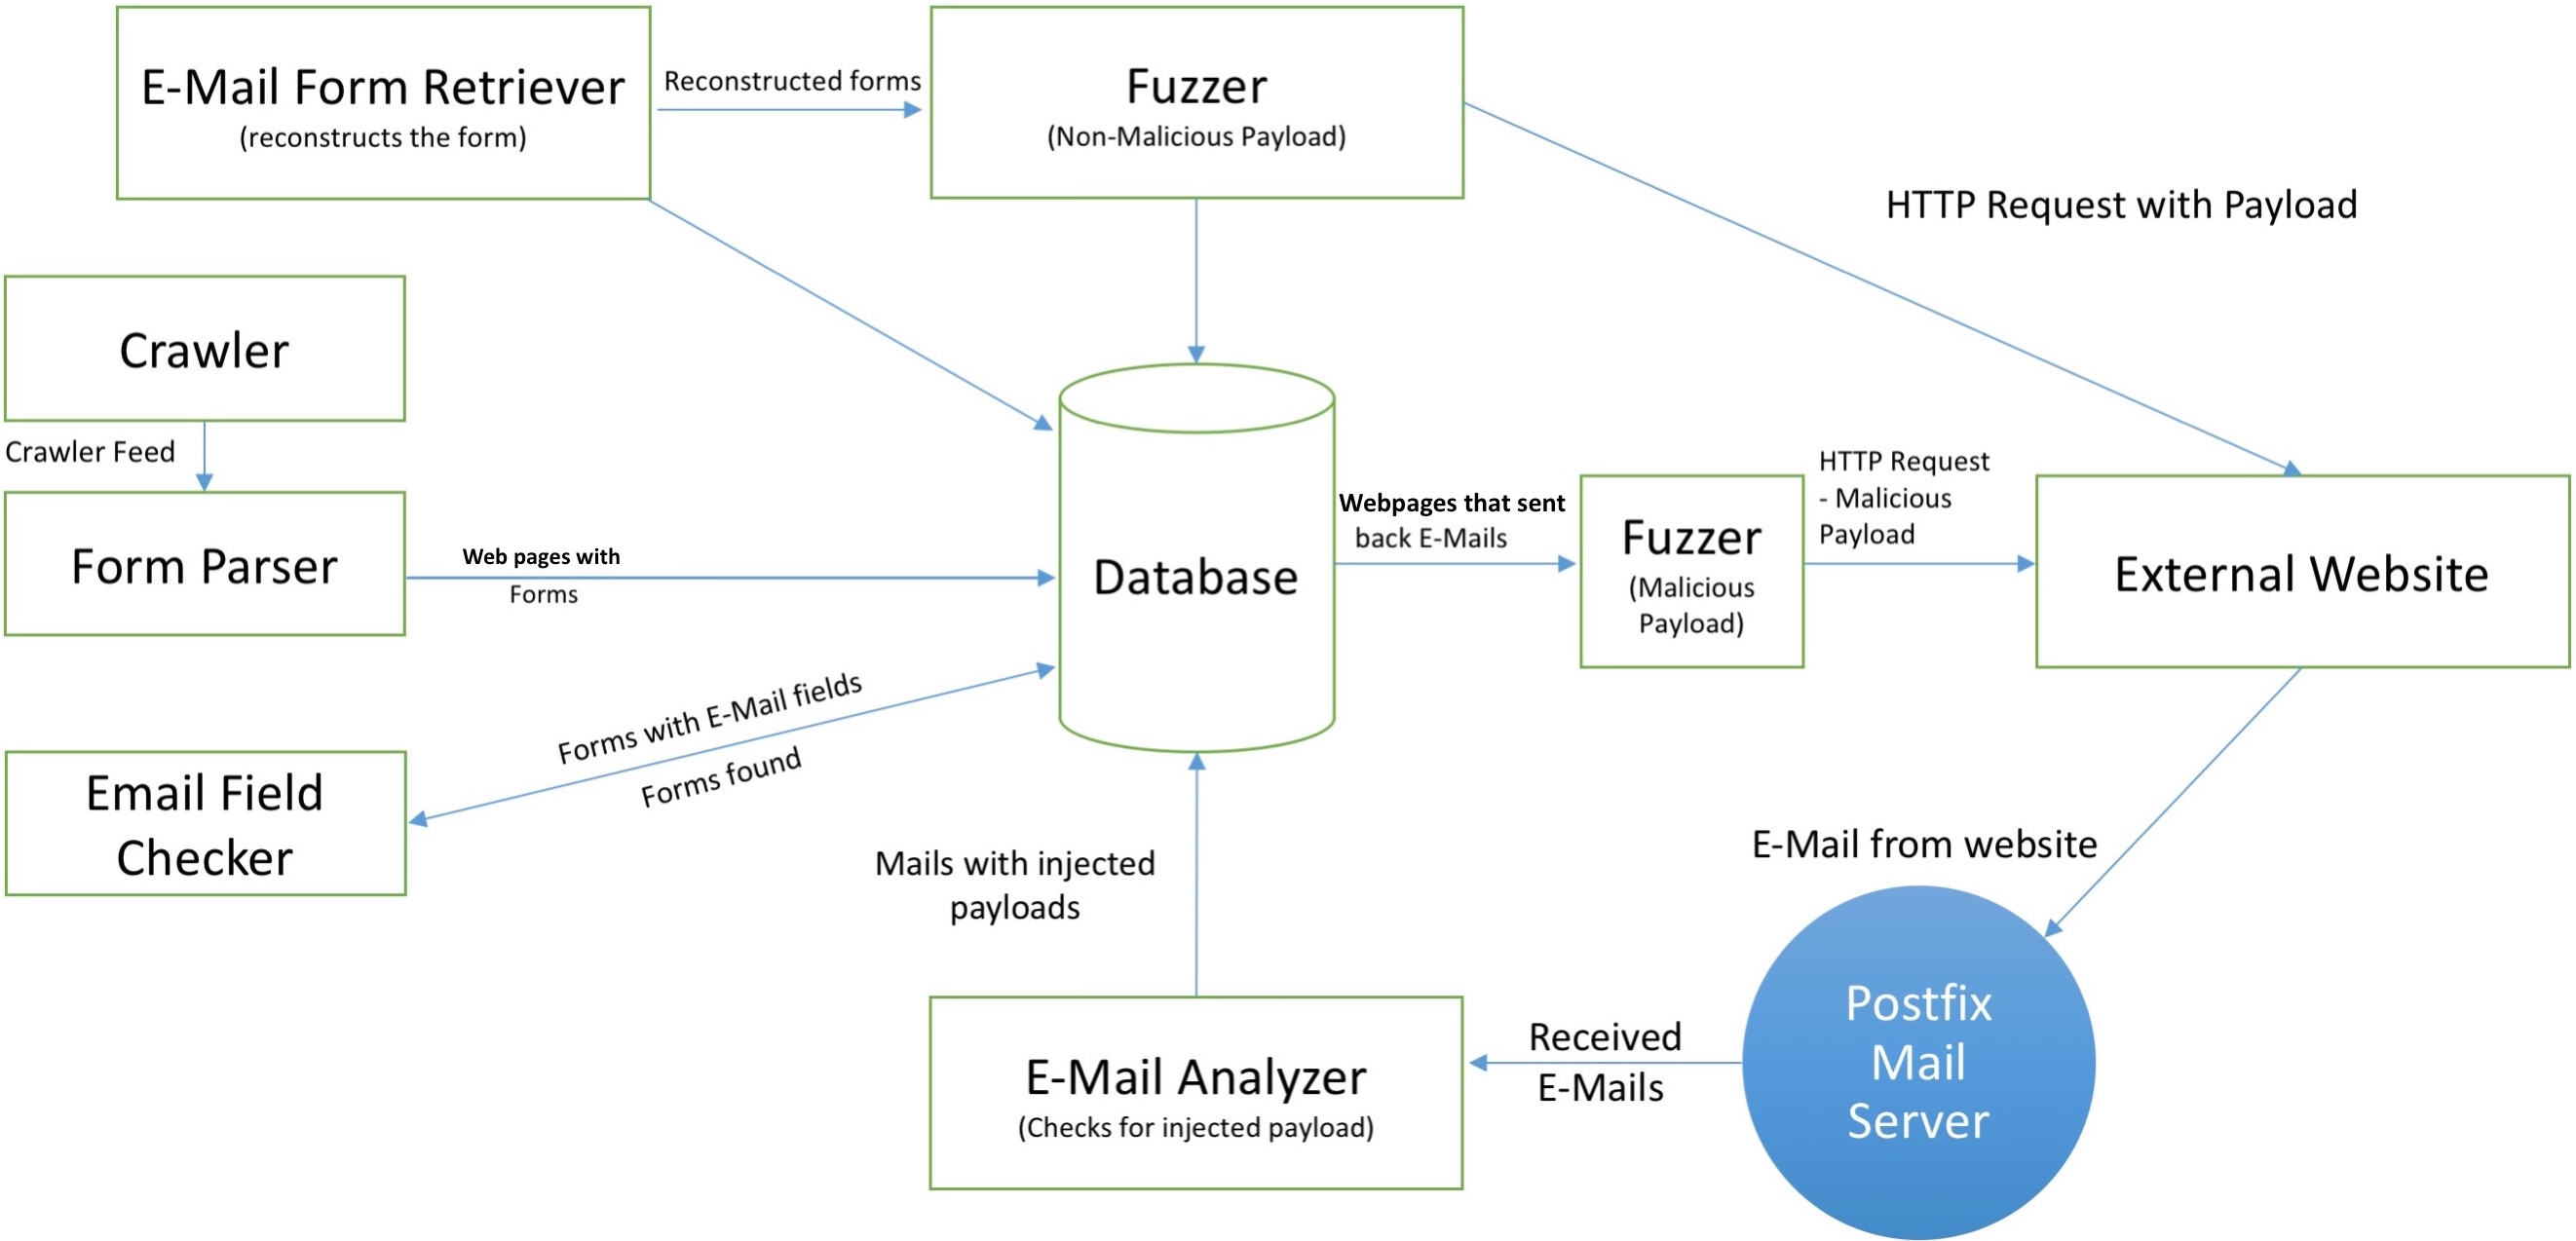
\includegraphics[width=.5\textwidth]{overall_crop}
	\caption{Overall system architecture.}
    \vspace{-5ex}
	\label{fig:overall}
\end{figure}

%\subsection{System Architecture}
\label{sys:arch}
Our system can be broadly divided into two modules: Data Gathering and Payload Injection.

The Data Gathering module is responsible for the following activities:
(1) Interface with the Crawler (Section~\ref{Comp:Crawler}) and
receive the URLs, (2) Parse the HTML for the corresponding URL and
store the relevant form data (Section~\ref{Comp:FP}), and (3) Check
for the presence of HTML forms that could allow a user to send/receive
\email and store references to these forms (Section~\ref{Comp:EMFC}).

    
The Payload Injection module is responsible for the following
activities: (1) Retrieve the HTML forms that could allow a user to
send/receive \email and reconstruct these forms
(Section~\ref{Comp:EMFR}), (2) Inject these forms with benign data
(non-malicious payloads) and generate an HTTP request to the
corresponding URL (Section~\ref{Comp:Fuzzer}), (3) Analyze the
received \emails, extracting the \email header fields and checking for
the presence of the injected payloads (Section~\ref{Comp:EMA}), and
(4) Inject the HTTP requests that sent us \emails with malicious
payloads, and generate an HTTP request to the corresponding URL to
check if an \ehi vulnerability exists in that web application
(Section~\ref{Comp:Fuzzer}).

	%% The functionality of each component is discussed further in the `Components' section (Section~\ref{Comp}). The Payload Injection pipeline is not a linear, but cyclic process, as we inject different payloads and analyze the received \emails.


\subsection{System Components}

\label{Comp}
\label{Comp:Crawler}
\label{Comp:EMFR}
\label{Comp:Fuzzer}
\label{Comp:EMA}
The Data Gathering module and Payload Injection modules are composed of smaller components. This section describes the functionality of those components.

\subsubsection{Data Gathering}
We used an open-source Apache Nutch based Crawler~\cite{nutch}. The \texttt{Crawler} provides the system with a continuous feed of URLs and the HTML contained in those pages. 
\label{Comp:FP}
The \texttt{Form Parser} is responsible for parsing the HTML and retrieving data about the HTML
forms on the page, including the following: (1) Form attributes, such
as \texttt{method} and \texttt{action} (URL) for the HTTP request, (2)
Data about form inputs, such as their attributes, names, and
default values. The default values are essential for fields like
{\lstinline{<input type="hidden">}} as these fields are usually used
to check for the submission of forms by bots, and (3) Presence of the {\lstinline{<base>}} element in the HTML, as this affects the final URL to which the form is to be submitted (if the \texttt{action} attribute is a relative URL).

\label{Comp:EMFC}
The \texttt{\Email Field Checker} is the final stage in the Data Gathering module. It receives the HTML form data and checks for the presence of \email fields in those forms. If any \email fields are found, it stores references to these forms.
The intuition here is that we do not want to try to fuzz all HTML forms on the web to look for \ehi vulnerabilities, rather just those HTML forms that are likely to invoke server-side email functionality.

The \Email Field Checker searches for the words \texttt{e-mail},
\texttt{mail} or \texttt{email} within the form, instead of an
explicit HTML5 \email field (e.g.,\ {\lstinline{<input type="email">}}). This is by design, taking into account a common
design pattern used by web developers, where they may have a text
field with an \texttt{id} or \texttt{name} attribute set to
\texttt{email}, instead of an actual \email type attribute, for
purposes of backward compatibility with older browsers. The output of this stage is stored in the database and acts as the input to the Payload Injection module.

%% Compared to searching for explicit \email fields, by searching for the presence of the words \texttt{\email}, \texttt{mail} or \texttt{email} in the form, we are assured very few false negatives. This is because our system is bound to find \email fields with their \texttt{type}, \texttt{name}, or \texttt{id} set to one of these words. The system is also substantially faster as we do not have to parse the individual form fields at this point in the pipeline. However, despite the advantages, this might also lead to a false positive rate. We discuss this possibility in detail in Section~\ref*{issues:fpr} - Design Issues.
\textbf{\Email Form Retriever} is the first stage in the Payload Injection
module. It does the following: (1) Retrieve forms and
remove duplicates, (2) reconstruct
each form's input fields and values from stored form data, and (3) construct the target URL
to create an HTTP request for fuzzing.

\textbf{Fuzzer}
% Adam: we should call these something else but modules. We already have the top two modules, which are composed of components, now we need to split these into something (not components again). - DONE
interacts directly with the external web applications. The system
injects payloads in two stages to reduce the total number of HTTP requests the system generates to detect an \ehi vulnerability. Making HTTP requests is an expensive process~\cite{httpperf}, and can cause bottlenecks in a Crawler-Fuzzer system~\cite{ShkapenyukTorstenSuel2001}.
The two different payloads used for fuzzing are:

\noindent\textbf{Non-Malicious Payload.}
The non-malicious payload is simply an \email address. The goal is to see if the web application will send an \email message based on our input. The specific format of the \email is \lstinline|reguser#@example.com|, where \texttt{\#} is replaced by an internal id that uniquely maps the payload to the form, and \texttt{example.com} is replaced by our domain.

\noindent\textbf{Malicious Payload.}
After receiving an \email from a specific form, we use the malicious payload to try to exploit an \ehi vulnerability. We inject the form fields with the \texttt{bcc} (blind carbon copy) header. If the vulnerability is present, this will cause the server to send a copy of the \email to the \email address we added as the \texttt{bcc} field.

We consider a special case: the addition of an \texttt{x-check:in} header field to the payloads. This is due to Python's exhibited behavior when attaching
headers. Instead of overwriting a header if it is already present, Python will ignore duplicate headers. So, if the \texttt{bcc} field is already present as part of the headers, our injected \texttt{bcc} header would be ignored. To overcome this, we inject a new header that is not likely to be generated by the web application. 

We created four different malicious payloads. Each of these payloads
is crafted for a particular use case. The four payloads are:
(1) nuser\#@example.com\textbackslash{}n\-bcc:\-maluser\-\#\-@example.com,
(2) nuser\#@\-example.com\textbackslash{}n\-bcc:\-maluser\-\#\-@example.com\textbackslash{}n\-x-check:in,
(3) nuser\#@\-example.com\textbackslash{}r\textbackslash{}n\-bcc:\-maluser\#\-@example.com,
and (4) nuser\#\-@example.com\-\textbackslash{}r\textbackslash{}n\-bcc:\-maluser\#\-@example.\-com\textbackslash{}r\textbackslash{}n\-x-check:in.
	
Payload 1 is the most minimal payload: it injects a newline character followed by the \texttt{bcc} field. Payload 2 contains the additional \texttt{x-check} header to inject Python-based web applications. Payloads 3 and 4 are added for purposes of cross-platform fuzzing: \texttt{\textbackslash{}r\textbackslash{}n} is the ``Carriage Return - New Line (CRLF)'' used on Windows systems~\cite{rfc2616}. The \# are replaced by an internal id, for mapping to the forms.

% Adam: If we need to cut things for space, we can cut this next line and the payload coverage table.

%\begin{table}[tbp]
%	\centering
%	\normalsize
%	\begin{tabular}{|c|c|c|}
%		\hline
%		\multicolumn{1}{|c|}{\textbf{Payload}} & \multicolumn{1}{c}{\textbf{Languages covered}} & \multicolumn{1}{|c|}{\textbf{Platforms covered}}\\
%		\hline
%		1 & PHP, Java, Ruby, etc. & Unix\\
%		\hline
%		2 & PHP, Java, Ruby, etc. & Windows\\
%		\hline
%		3 & Python & Unix\\
%		\hline
%		4 & Python & Windows\\
%		\hline
%	\end{tabular}
%	\caption[\titlecap{Payload coverage}]{Payload coverage, each payload covers a different platform/language.}
%	\label{tab:payloadcov}
%\end{table}

%% \begin{table}[tbp]
%% 	\centering
%% 	\scriptsize
%% 	\begin{tabular}{|c|c|c|}
%% 		\hline
%% 		\multicolumn{1}{|c|}{\textbf{Language/Platform}} & \multicolumn{1}{c}{\textbf{Unix}} & \multicolumn{1}{|c|}{\textbf{Windows}}\\
%% 		\hline
%% 		\textbf{PHP, Java, Ruby} & 1 & 3\\
%% 		\hline
%% 		\textbf{Python} & 2 & 4\\
%% 		\hline
%% 	\end{tabular}
%% 	\caption[\titlecap{Payload coverage}]{Payload coverage, each payload covers a different platform/language.}
%% 	\label{tab:payloadcov}
%% \end{table}

Along with the payload, the Fuzzer also injects data into the other fields of the form. This data must pass validation constraints on the individual input fields (e.g.,\ name field might not be allow numbers).  As crawling and fuzzing input fields on the web is an open problem~\cite{raghavan2000crawling}, we chose to go with a best-effort approach. To maximize the amount of vulnerabilities the system discovers, the data injected into the input fields should adhere to the constraints. The Fuzzer uses a ``Data Dictionary'' which has predefined ``keys'' and ``values'' for standard input fields such as \texttt{name}, \texttt{date}, \texttt{username}, \texttt{password}, \texttt{text}, and \texttt{submit}.
The values for these are generated for each form, based on generally followed guidelines for such fields. For example, password fields should consist of at least one uppercase letter, one lowercase letter, and special characters.

When the fuzzed data is ready, the Fuzzer constructs the appropriate HTTP request (GET or POST) and sends the HTTP request to the URL that was generated by the \Email Form Retriever (Section~\ref{Comp:EMFR}). 


\textbf{Injection Verification}
module checks for the presence of injected data in the received \emails. This module works on the \emails received and stored by our Postfix server, and, depending on the user account that received the \email, it performs different functions.

\noindent\textbf{Analyzing regular e-mail.}
\sloppy
`Regular \email' refers to the \emails received by account {\lstinline{reguser#@example.com}} that were sent due to injecting the regular, non-malicious, payload (discussed in Section~\ref{Comp:Fuzzer}). The objective of the analysis on this \email is identify if the input fields that we injected with data appear on the resulting \email, and if so, which fields appear where.

To find this, we parse each received \email, and check whether \emph{any} of the fields we injected with data appear in either the headers or body of the \email. These could be fields such as name, username, age, etc. If they do, we add them to the list of fields that can \emph{potentially} result in an \ehi vulnerability for the given \email. 

We then pass on this information back to the Fuzzer pipeline, along with the vulnerable form, where these fields are \emph{also} fuzzed along with the \email fields to check for the presence of \ehi.

\noindent\textbf{Analyzing \email with payloads}
The ``\emails with payloads'' refers to \emails received by either the {\lstinline{nuser#@example.com}} or {\lstinline{maluser#@example.com}} accounts. These \emails could only be received as a result of injecting the malicious payloads that were discussed in Section~\ref{Comp:Fuzzer}. 

\noindent\textbf{Detecting injected \texttt{bcc} headers}
As discussed in the payloads Section~(\ref{Comp:Fuzzer}), the payloads were crafted such that the \emails received by the \texttt{maluser} account directly indicate the presence of the injected \texttt{bcc} field. 

\label{analyze:detect_x_check}
\noindent\textbf{Detecting injected \texttt{x-check} headers} \Emails
not received by the \texttt{maluser} account but by the \texttt{nuser}
account constitute a special category of \emails. These \emails could
have been generated due to two reasons: (1) The web application
performed sanitization and stripped out the \texttt{bcc}
part of the payload, thereby sending \emails only to the
\texttt{nuser} account. These \emails then act as proof that the
vulnerability was not found on the given URL. (2) The \texttt{bcc}
header can be ignored for other reasons (e.g.,\ Python's default
behavior when it encounters duplicate headers). In this case, we check
if the \email contains the custom header \texttt{x-check}. If it does,
then this is a successful exploit of the vulnerability.




\section{Evaluation}

We ran our system on the web at large, attempting to discover \ehi
vulnerabilities in web applications. We used as a seed to
\texttt{Crawler} the Alexa top 10,000 websites as well as a feed of
10,000 random blog pings per day from \url{weblogs.com}. All domains
were crawled to a maximum depth of four, and the crawler respected the
\texttt{robots.txt} directive. This seed enabled \texttt{Crawler} to
get an overview of not only the popular websites (from the Alexa top
10k) but also the long-tail of blog posts and websites that they
linked to.


From our extensive crawl of the web, we were able to gather the data
shown in Table~\ref{tab:data}. We ran the system for 76 days, during which our system crawled \urls unique URLs,
and found a total of \forms\ forms from \uniqueforms\ unique domains. Out of these forms, our system
found \emailforms\ forms that contained an \email field, from \uniqueemailforms\ unique domains.
Table~\ref{tab:fuzzed_data} shows the quantity of \emails we received for the benign and malicious payloads. 
\begin{table}[tbp]
	\centering
	\scriptsize
	\begin{tabular}{|c|c|}
		\hline
		\multicolumn{1}{|c|}{\textbf{Type of Data}} &
		\multicolumn{1}{c|}{\textbf{Quantity}}\\
		\hline
		URLs Crawled & \urls \\
		\hline
		Total Forms found & \forms \\
		\hline
		Forms with E-Mail Fields & \emailforms \\
		\hline
	\end{tabular}
	\caption[\titlecap{Collected data}]{The data collected for our
      project.}
    \vspace{-5ex}
	\label{tab:data}
\end{table}

\begin{table}[tbp]
	\centering
	\scriptsize
	\begin{tabular}{|c|c|c|}
		\hline
		\multicolumn{1}{|c|}{\textbf{Type of fuzzing}} &
		\multicolumn{1}{c|}{\textbf{Forms fuzzed}} &
		\multicolumn{1}{c|}{\textbf{E-Mails received}}\\
		\hline
		Regular payload & \fuzzed & \recd \\
		\hline
		Malicious payload & \malfuzzed & \success \\
		\hline
	\end{tabular}
	\caption[\titlecap{Fuzzed data}]{The data we fuzzed and the e-mails we received.}
    \vspace{-5ex}    
	\label{tab:fuzzed_data}
\end{table}


\noindent\textbf{\Email received from forms.} The \emails that we
received can be categorized into two categories. (1) \Emails due to
regular payload: This represents the total number of web applications
that sent \emails to us. This indicates that we were able to
successfully submit the forms on these sites to trigger the web
application to send an \email. (2) \Emails due to malicious payload:
Once we receive an \email from a web application due to the regular
payload, we fuzz those forms with the malicious payloads. This field
represents the total number of unique URLs that contain an \ehi
vulnerability.


%%Table~\ref{tab:fuzzed_data} shows the quantity of \emails that we received for the benign and malicious payloads. 
%\begin{table}[tbp]
	\centering
	\scriptsize
	\begin{tabular}{|c|c|c|}
		\hline
		\multicolumn{1}{|c|}{\textbf{Type of fuzzing}} &
		\multicolumn{1}{c|}{\textbf{Forms fuzzed}} &
		\multicolumn{1}{c|}{\textbf{E-Mails received}}\\
		\hline
		Regular payload & \fuzzed & \recd \\
		\hline
		Malicious payload & \malfuzzed & \success \\
		\hline
	\end{tabular}
	\caption[\titlecap{Fuzzed data}]{The data we fuzzed and the e-mails we received.}
    \vspace{-5ex}    
	\label{tab:fuzzed_data}
\end{table}

%
%\noindent\textbf{\Email received from forms.} The \emails that we
%received can be categorized into two categories. (1) \Emails due to
%regular payload: This represents the total number of web applications
%that sent \emails to us. This indicates that we were able to
%successfully submit the forms on these sites to trigger the web
%application to send an \email. (2) \Emails due to malicious payload:
%Once we receive an \email from a web application due to the regular
%payload, we fuzz those forms with the malicious payloads. This field
%represents the total number of unique URLs that are contain an \ehi
%vulnerability.


\subsection{Analysis of the Received \Email Data}

During our analysis of the received \emails, we found that the \emails that we received belonged to three categories:

(1) \Emails with the \texttt{bcc} header successfully injected. This form
of injection was our initial objective, and we found
% Adam: Sai, why isn't this number a command? - DONE.
\ehibcc such \emails in our received \emails. This validates that the
web applications that sent these \emails are vulnerable to \ehi.
	
(2) \Emails with the \texttt{To} header successfully injected. We
discovered an unintended vulnerability class during our analysis,
which we call \texttt{To~header injection}. These injections reflect
the ability to inject any number of \email addresses into the
\texttt{to} field of the SMTP message while being unable to inject any
other header into the \emails. We found \ehito such \emails in our
received \emails. We attribute this behavior to inconsistent
sanitization by the application.
   
While not allowing us complete control over content of the \emails
sent, \texttt{To header injection} makes it possible to append any
number of \email addresses, thereby enabling us to leak information or
perform DoS (Denial of Service) attacks against the web application.
	
(3) \Emails with the \texttt{x-check} header successfully injected. The
third category of \emails received were \emails with the
\texttt{x-check} header injected. As discussed in
Section~\ref{analyze:detect_x_check}, we can differentiate between
unsuccessful attempts and successful attempts by injecting the
additional header and checking whether headers other than the
\texttt{bcc} header can be injected into the generated \email.
\ehixcheck \emails were received with the \texttt{x-check} header
injected.

% Adam: Sai, we need to put the actual numbers in the text. We cannot count on the readers to look at the table (of course, we should use the commands
We list each category and the number of \emails received by that
category in Table~\ref{tab:analysis}. We explain the combination of
these header injections (4-7) as follows:

%\begin{table}[tbp]
\begin{wraptable}{r}{6.5cm}
	\centering
	\scriptsize
    \vspace{-4ex}
	\begin{tabular}{|l|p{1cm}|}
		\hline
		\textbf{Type of Injection} & \textbf{\# e-mails}\\
		\hline
		E-Mail Header Injections with \texttt{bcc} header & \ehibcc \\
		\hline
		E-Mail Header Injections with \texttt{x-check} header & \ehixcheck \\
		\hline
		\texttt{To header} injections alone & \ehito \\
		\hline
		Injections with both \texttt{bcc} and \texttt{x-check} headers & \ehibccxcheck \\
		\hline
		Both \texttt{To header} injections and x-check headers &
		\ehitoxcheck \\
		\hline
		\texttt{x-check} headers found in \texttt{nuser} e-mails & \ehinuserxcheck \\
		\hline
		Unique \texttt{x-check} headers found in \texttt{nuser} e-mails & \ehiuniquenuserxcheck \\
		\hline
		Total successful injections (1 + 3 + 7) & \success \\
		
		\hline
	\end{tabular}
	\caption[\titlecap{Analysis of the data}]{Classification of the e-mails that we received into broad categories of the vulnerability.}
    \vspace{-5ex}
	\label{tab:analysis}
    %\end{table}
\end{wraptable}


\Email Header Injections with both \texttt{bcc} and \texttt{x-check}
headers: These represent the scenario where an attacker can inject
multiple headers into the \emails. We can see that 54\% of the
received \texttt{bcc} header injected \emails are also susceptible to
being injected with additional headers.
      % Adam: What is the exact percentage? We should use that rather than an approximate number - DONE.
	
Both \texttt{To} header injections and \texttt{x-check} headers: This
combination shows us that in addition to being able to inject into the
\texttt{To} fields, we injected additional headers into the \email. It
is not clear what causes this behavior; however, these can be
exploited to achieve the same result as a regular \ehi.
	
Total \texttt{x-check} headers and unique \texttt{x-check} headers
found in \texttt{nuser} \emails: We found a total of \ehinuserxcheck
\emails in the \texttt{nuser} account. Out of these,
\ehiuniquenuserxcheck had unique form ids that were \emph{not} already
found in the \texttt{maluser} account. We attribute these \emails to
(probably) being sent by a web application that was built with Python
or another language having a similar behavior with respect to ignoring
duplicate headers while constructing an \email, thus appending the
\texttt{x-check} header and \emph{not} the \texttt{bcc} header.
      % Adam: What is the actual behavior? This is confusing. - Changed. DONE.
	
Total successful injections: This represents the total number of
successful injections. This includes the \ehi with \texttt{bcc}
header\,(1), \texttt{To} header injections\,(3), and Unique
\texttt{x-check} headers found in \texttt{nuser} \emails\,(7). A total
of \success vulnerabilities were found by our system.

      % Adam: we need the actual #s here too. These are the core results of our analysis, they need to be in the text. - DONE.


\subsection[The Pipeline]{Understanding the Data Pipeline}

%This section serves to represent our pipeline quantitatively and graphically. 
Table~\ref{tab:pipeline} shows the data gathered by our pipeline, with the differential changes at each stage of the pipeline. At each stage of the pipeline, the amount of data decreases, for instance, out of the \urls\ URLs we crawled, only \forms\ forms (\formsDelta) were found. Out of these, only \emailforms\ forms (\emailformsDelta) contained e-mail fields.

In our fuzzing attempts, the same behavior is observed. We fuzzed \fuzzed\ forms with the regular payload, which resulted in a total of \recd\ e-mails~(\recdDelta). After analysis of the received e-mails, we further fuzzed \malfuzzed\ forms, which resulted in \success\ e-mails (\successDelta) which contain the vulnerability across \ips IP addresses from \domains domains.

We attribute the difference in the number of forms found to the number of forms fuzzed (a difference of \diffFoundFuzz forms) to the presence of bot-blocking mechanisms on a website (discussed in Section~\ref{limitations}), though we do not know what percentage was caused by each bot-blocking mechanism discussed in Section~\ref{limitations}. 

Note that over 1\% of the forms that were not fuzzed (100 out of \diffFoundFuzz) were also tested manually using PostMan to generate HTTP requests with payloads to verify that our system was working as intended.

\begin{table}[tbp]
%\begin{wraptable}{r}{7cm}
	\centering
	\scriptsize
	\begin{tabular}{|l|c|c|}
		\hline
		\textbf{Pipeline Stage} & \textbf{Quantity} & \textbf{Differential}\\
		\hline
		Crawled URLs  & \urls & $\Delta$ d2/d1 * 100 \\
		\hline
		Forms found  & \forms & \formsDelta \\
		\hline
		E-Mail Forms found  & \emailforms & \emailformsDelta \\
		\hline
		Fuzzed with regular payload  & \fuzzed & \fuzzedDelta \\
		\hline
		Received e-mails  & \recd & \recdDelta \\
		\hline
		Fuzzed with malicious payload  & \malfuzzed & \malfuzzedDelta \\
		\hline
		Successful attacks  & \success & \successDelta \\
		\hline

	\end{tabular}
	\caption[\titlecap{Data gathered by our pipeline}]{Data gathered
      by our pipeline at each stage}
    
	\label{tab:pipeline}
\end{table}
%\end{wraptable}



% Adam: this is an important part of our contribution, but I don't think that it belongs here. 
%% From our research, it is clear that E-Mail Header Injection is quite widespread as a vulnerability, appearing on \successDelta\ of forms that we were able to perform automated attacks on. This value acts as a lower bound for E-Mail Header Injection vulnerability, and can quite easily be much more if the attacks were of a more concentrated nature, crafted for the individual websites and less automated.

\subsection{Analysis of Vulnerable domains}

We performed the following analyses on the vulnerable domains:
\begin{itemize}
	\item Checking Alexa rankings of the vulnerable domains.
	\item Investigating the back-end languages used by the vulnerable domains.
	\item Analyzing the presence of DKIM (DomainKeys Identified Mail), SPF (Sender Policy Framework), and DMARC (Domain-based Message Authentication, Reporting \& Conformance) mechanisms on these domains.
\end{itemize}


\subsubsection{Alexa rankings of vulnerable domains.}
We searched through the Alexa rankings data\cite{alexa} for the domains that were found to be vulnerable, and found 135 of these domains in the top 1 million ranked websites. A detailed distribution of the rankings is shown in Table~\ref{tab:alexa} / Figure~\ref{fig:alexa_data_bar} / Figure~\ref{fig:alexa_data_pie}.

%TODO Adam: Need to decide if table or graph, if graph, then Pie vs Bar.
%\begin{table}[tbp]
%	\centering
%	\scriptsize
%	\begin{tabular}{|l|c|}
%		\hline
%		\textbf{Alexa Ranking Ranges} & \textbf{Vulnerable domains} \\
%		\hline
%		0-5K & 1 \\
%		\hline
%		5-50k & 7 \\
%		\hline
%		50k-100k & 6 \\
%		\hline
%		100k-250k & 23 \\
%		\hline
%		250k-500k & 30 \\
%		\hline
%		500k-1m & 68 \\
%		\hline		
%	\end{tabular}
%	\caption[\titlecap{Distribution of vulnerable domains based on Alexa Rankings}]{Distribution of vulnerable domains based on Alexa Rankings}
%	\vspace{-5ex}
%	\label{tab:alexa}
%\end{table}

\begin{figure}
	\centering
	\begin{minipage}{.5\textwidth}
		\centering
		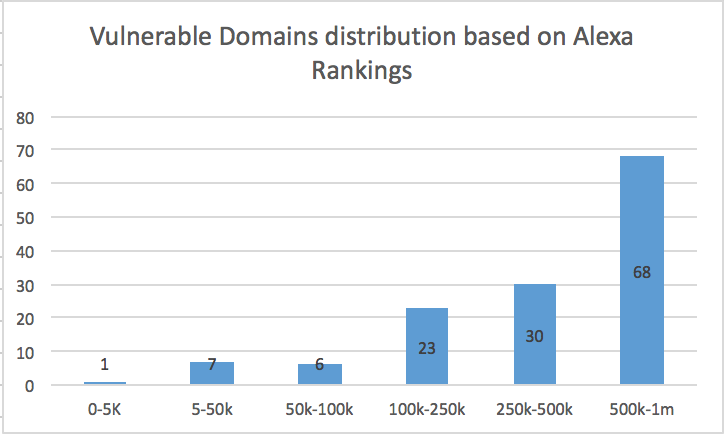
\includegraphics[width=.95\linewidth]{alexa_data_bar}
		\captionof{figure}{Distribution of vulnerable domains based on Alexa Rankings}
		\label{fig:alexa_data_bar}
	\end{minipage}%
	\begin{minipage}{.5\textwidth}
		\centering
		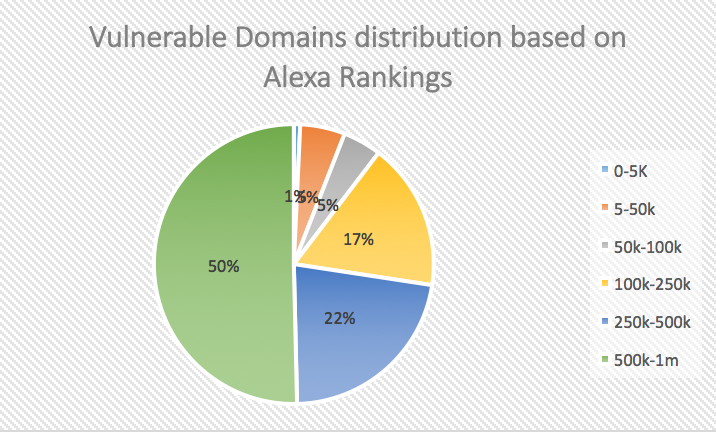
\includegraphics[width=.95\linewidth]{alexa_data_pie}
		\captionof{figure}{Distribution of vulnerable domains based on Alexa Rankings}
		\label{fig:alexa_data_pie}
	\end{minipage}
	\vspace{-1.5ex}
\end{figure}


%TODO Adam: Is a table/graph for backend technologies needed?
% apparently \subsubsection need to have a period at the end.
\subsubsection{Back-end technologies of vulnerable domains.}
We investigated the top 100 vulnerable domains on our list (based on the alexa rankings) to find the back-end technologies used by these vulnerable domains to see if there was any recurring pattern. Using BuiltWith~\cite{builtwith} and wappalyzer~\cite{wappalyzer}, we found that a majority of the vulnerable domains (79\%) used PHP as one of the back-end technologies, while 17\% of domains used WordPress and another 14\% used ASP.Net. Other technologies used include Java (5\%), Ruby on Rails (1\%), and Perl (1\%). We also found a combination of other technologies like Magento, CakePHP, CodeIgniter, Joomla, mail.ru and Drupal being used in conjunction with one of the above languages. A point to be noted is that 4\% of the websites also used Contact Form 7~\cite{CF7}, which is supposed to protect against such attacks. 

\subsubsection{Presence of e-mail spoofing protection on vulnerable domains.}
\subsection{Exploitation Evidence}

We compared the \ips IPs that our system found to be vulnerable to \ehi against 13 well-known IP blacklists, to see if these IPs were being exploited by attackers to send spam. The blacklists that we used were: 
\texttt{zen.spamhaus.org},
\texttt{spam.abuse.ch},
\texttt{cbl.abuseat.org},
\texttt{virbl.dnsbl.bit.nl},
\texttt{dnsbl.inps.de},
\texttt{ix.dnsbl.manitu.net},
\texttt{dnsbl.sorbs.net},
\texttt{bl.spamcannibal.org},
\texttt{bl.spamcop.net},
\texttt{dnsbl-1.uceprotect.net},
\texttt{dnsbl-2.uceprotect.net},
\texttt{dnsbl-3.uceprotect.net},
\texttt{db.wpbl.info}.

We found that \ipsblacklist of these IPs were blacklisted on at least one of the above blacklists for sending out spam, and \ipsblacklistmulti of them were found on multiple blacklists. We do not have enough data to make an observation about whether these attackers are exploiting \ehi to send out the spam, as an alternative hypothesis is that these IPs are on the blacklists because the server has different vulnerabilities that attackers exploit to cause the server to send spam (assuming that the server is normally benign).  

\subsection{Emails with Malicious Attachments}
As additional analysis to find domains on the internet that send out malicious attachments, we checked the \emails received by the `reguser' account (which are injected with regular \email addresses and not malicious data) for the presence of attachments that may contain malicious software, which will indicate that the server itself is not benign. 

To do this, we passed the \totalattachmentcount attachments we received to VirusTotal~\cite{virustotal} -- an online malware scanner that checks for the presence of malware by running 40+ virus scanners on the uploaded files. We found that out of the \totalattachmentcount attachments, \totalvirusemails were malicious, out of which \totalvirusattachmentcount were from unique domains. This data is just a by-product of our research and could very well lead to future research.
%It is to be noted that none of these domains were found on the spam analysis we did earlier, indicating that if these could be exploited, we could send emails with malicious attachments to other people using these servers.

\subsection{Responsible Disclosure of Discovered Vulnerabilities}
After we discovered an \ehi vulnerability on a particular website, we attempted to notify the developers of the vulnerable web application, along with a brief description of the vulnerability.
We chose to \email the following mailboxes, following the rules
specified in RFC~2142~\cite{rfc2142}: \texttt{security@domain.com},
\texttt{admin@domain.com}, and \texttt{webmaster@domain.com}
 
Out of the \domains\ vulnerable domains found, only
\emailedDefaultmailbox websites had the mailboxes able to receive
\emails. For the remaining domains, we used the
\texttt{whois}~\cite{whois} data to find the contact details of the
owner and then \emailed them. We received \responses developer
responses, confirming \confirmed discovered vulnerabilities. Four of
the developers fixed the vulnerability on their website.

From our research, it is clear that \ehi is quite widespread as a
vulnerability, appearing on \successDelta\ of forms that we were able
to perform automated attacks on. This value acts as a \emph{lower
  bound} for prevalence of \ehi vulnerability, and can quite easily be
larger if the attacks were broader, crafted for the individual web
application, and less automated.


%% \begin{table}[tbp]
%% \centering
%% \scriptsize
%% \begin{tabular}{|c|c|c|}
%% 	\hline
%% 	\multicolumn{1}{|p{2cm}}{\centering \textbf{Notified websites}} &
%% 	\multicolumn{1}{|p{2cm}|}{\centering \textbf{Developer Responses}} &
%% 	\multicolumn{1}{p{2cm}|}{\centering \textbf{Confirmed discoveries}}\\
%% 	\hline
%% 	\domains\ & \responses & \confirmed \\
%% 	\hline
%% \end{tabular}
%% 	\caption[\titlecap{}]{Responsible disclosure of the discovered vulnerabilities to developers and the number of received responses.}
%% 	\label{tab:devresp}
%% \end{table}

% Adam: did we get updated notifications? - updated. DONE.



\section{Discussion}
\vspace{-2ex}
    In this section, we discuss the lessons learned, the limitations of our system, and how to mitigate \ehi vulnerabilities.
\subsection{Lessons Learned}
\vspace{-1ex}
From our results, it is evident that \ehi vulnerabilities exist in the wild.
% Adam: Sai, I don't understand this math. The 1.46% number is calculated based on the number of forms we were able to fuzz with a malicious payload. This isn't the same as the number of websites. But, using 673/21675680 is not good either because that is # of URLs and it seems like the number you have here is websites. What we need is what % of *websites* (probably estimated as domains) did we find to be vulnerable out of *all* websites/domains that we found. When we use this number, we need to be clear what it is that we are using. -- FIxed this to be clear.
Despite its relatively low occurrence rate compared to the more popular SQL Injection and XSS (Cross-Site Scripting), when we consider total number of domains on the World Wide Web--- 1,018,863,952 according to Internet Live Stats~\cite{InternetLiveStats2016} as of early 2016---and calculate \successWebsitesDelta percent (the occurrence rate of \ehi vulnerability calculated from vulnerable domains as found by our system to total number of domains crawled) of that number, this yields 295,693 domains. Of course, extrapolation in this way is not an accurate measure of the prevalence of \ehi vulnerabilities. However, even with as few as a thousand domains affected by this vulnerability, it can still have a disastrous impact on these domains, and also on overall World Wide Web due to the traffic caused by the sheer number of generated e-mails. 
    
%% We believe that one of the reasons for the small percentage of occurrence (compared to SQL Injection or Cross-Site Scripting), can be attributed to what we like to call the `car parking analogy'.
%%     The car parking analogy is something like this: Imagine that we are parking a car on a road that is prone to attacks by thieves. Now, if all the cars were unlocked, the car that is most likely to get stolen is quite unsurprisingly the most expensive one or the one that is easiest to get away with.
    
%%     Now imagine the same thing on the World Wide Web: we have websites that can each have multiple vulnerabilities. Now, it makes sense for an attacker to try and attack websites with more widespread vulnerabilities such as SQL Injection or XSS, rather than attempt to exploit E-Mail Header Injection, seeing as this requires a more concentrated effort, with carefully crafted payloads and a waiting time for the e-mail to be delivered. SQL Injection attacks and XSS attacks are also better documented, with well-known attack vectors, and automated tools to help detect the presence of these vulnerabilities on websites.
    
%%     This also gives more incentive for the website developer to add protection against attacks such as SQL injection and XSS. The developer might then (possibly with the help of a sanitization library) sanitize the user input and remove \emph{all} special characters, including the newline characters (\textbackslash{}n, \textbackslash{}r), which adversely affects E-Mail Header Injection attacks.

%% 	We come to this conclusion because of our discovery of the \texttt{To header injection}. Clearly, this is possible due to incomplete sanitization performed by the application. We suspect that this incomplete sanitization is actually sanitization that is performed for some other vulnerability, and not specifically for E-Mail Header Injection attacks. We would also like to remark that \texttt{To header injection} is not complete E-Mail Header Injection, but only a special subset.
	
%%     Thus, indirectly, this kind of protection against other attacks affects the attempts to perform E-Mail Header Injection. However, this does not completely negate the attempts if the checks are only on the client-side. Also, even with server-side validation, often, the only input fields that are validated are ones that are either inserted into the database (SQL Injection) and the ones that are displayed to the user as part of the web site (XSS).

% Adam: Please add a citation to a CAPTCHA paper - DONE.
	
	%% This does not mean that the vulnerability is not a large threat. In fact, this vulnerability can also have some major consequences, the least of which can be spamming and phishing attacks.
	%% In today's digital world, identity theft has become all the more common. E-Mail Header Injection provides attackers with the ability to easily extract information about users, not just from a server, but from the user himself, by sending him fake messages that look extremely authentic, since these messages are sent by the mail server of the website itself.
    
    We found two different forms of \ehi: the first one is the traditional one, injecting any header into the \email that allows the attacker complete control over the contents of the \email. 
The second attack has not yet been documented and provides the ability to inject multiple \email addresses into the \texttt{To} field. We call this a \texttt{To header injection}. In this  vulnerability, an attacker can add addresses to the \texttt{To} field of the email with newlines separating the \email addresses. We could not determine if this vulnerability is due to unique flaws in each web application or if this vulnerability is due to an implementation issue with a particular language or framework. However, from our preliminary analysis, it is evident that the vulnerable web applications do not share much in common. 

\texttt{To header injection} allows an attacker to extract information that should be private,
% Adam: It's not clear what this means that we have enough data to spoof the few lines of the message. I thought to header injection just controls the TO field, not the message contents. - Fixed, my bad. DONE.
and in some of these cases, able to inject enough data to spoof other headers of the \email message. From Table~\ref{tab:analysis}, information leakage using \texttt{To header injection} was possible on \ehito forms, while spoofing using \texttt{To header injection} was possible on \ehitoxcheck forms.
    
    %% While not being as impactful as the primary vulnerability, this form of the vulnerability does still provide the ability to send \emails to multiple recipients, and can easily result in information leakage or spam generation on a large scale.
    

\subsection[Limitations]{Limitations}
\vspace{-1ex}
\label{limitations}
		Because our system is fully automated, it is also susceptible to being stopped by mechanisms in web applications that prevent automated crawls or form submissions. A common reason for our fuzzing attempts to fail is the bot-blocking mechanisms built into the web applications. CAPTCHAs (Completely Automated Public Turing test to tell Computers and Humans Apart)~\cite{captchas2} pose a very difficult problem for our system to exploit \ehi, even if it is present.
		Other measures such as hidden form fields and CSRF (Cross-site Request Forgery~\cite{csrf}) tokens are also often used to detect bots~\cite{captchas3,captchas2}.

		We made sure that we do not fuzz hidden fields in the form, and as our system does not depend on authenticated sessions, CSRF tokens do not pose an issue. However, despite considerable active research in breaking CAPTCHAs~\cite{captchas2,captchas}, breaking CAPTCHAs remains out of the scope of this project. 
		
	   Due to the growing emphasis on responsive web applications, more and more web applications are being built with only client-side JavaScript. Even conventional web applications use JavaScript to dynamically insert content and update the pages. This trend means that these dynamically injected HTML components are not part of the initial HTML that is sent to the client by the server.

       		\begin{wraptable}{r}{7.4cm}
%		\begin{table}[tb]
			\centering
			\scriptsize
			\begin{tabular}{|p{4cm}|c|c|}
				\hline
				\multicolumn{1}{|c}{\textbf{Method}} &
				\multicolumn{1}{|c|}{\textbf{Running time}} &
				\multicolumn{1}{|c|}{\textbf{Slowdown}}
				\\
				\hline
				\centering Using our pipeline & 629.043 & - \\
				\hline
				\centering Our pipeline with Selenium & 919.372 & \slowSelenium \\
				\hline				
				\centering Parsing \email fields instead of `grep'ing& 707.154 & \slowParse \\								
				\hline
			\end{tabular}
			\caption[\titlecap{}]{Running times in seconds for crawling, parsing, and detecting presence of \email fields in 1000 random web pages.}
            \vspace{-5ex}
			\label{tab:perf}
            %		\end{table}
        \end{wraptable}

		Thus, our system will not see dynamically injected forms and hence is unable to detect if \ehi vulnerabilities are present in these forms. The workaround would be to use a JavaScript engine to query for the \texttt{document.getElementsByTagName('html')[0].innerHTML} (from inside web browser automation tools such as Selenium), then use that as the source HTML. 
		
		A comparison of the running times between the different approaches is shown in Table~\ref{tab:perf}. We chose not to use Selenium as it results in a slowdown of \slowSelenium. 


        Because we search for the words \texttt{e-mail}, \texttt{mail}, or \texttt{email} within the HTML form, if the website does not use English names for its forms, our system will not be able to find the presence of an \email field. An example is by using the French word for \texttt{e-mail}---courrier {{\'e}}lectronique--- our system is unable to find the presence of the e-mail field. 
        
		During the crawl, our system was blacklisted by a few web
        applications (mostly WordPress ones), and Internet Service
        Providers (ISPs). To overcome this, we did two things: (1)
        used an IP range of 60 different IP addresses, and (2) Used a
        blacklist of our own to prevent our Fuzzer from fuzzing
        applications that are known to blacklist automated crawlers.
        This restricted us from gathering data about these
        applications.


		We found that certain WordPress plugins prevent the \ehi attack by sanitizing user input on contact forms. Although not all  WordPress web applications are secure, between the presence of the plugins on some websites, and getting tagged as ``spambots'' by others, we found few vulnerabilities on WordPress web applications.

        E-Mail libraries such as the PHP Extension and Application Repository's (PEAR) mail library provide sanitization for user input. While this is not strictly a limitation of our project, it still means that we are not able to inject sites that used these libraries.

        The parser that we use for HTML parsing---Beautiful Soup---does not parse heavily malformed HTML and throws an exception on encountering such HTML. Thus, we have designed the system to exit gracefully on such occasions. A side-effect of this is that our system is unable to test web applications with very bad HTML markup.

        Black-box testing is highly beneficial as explained in Section~\ref{sys:appr}, however it also has a drawback in that we cannot verify whether the reported vulnerability exists in the source code or is a feature of the website (e.g., the website allows users to send bulk e-mail, adding many \texttt{cc} or \texttt{bcc} headers). We must manually notify the developers to get this feedback.

%%        	As discussed in Section~\ref{Comp:EMFC}, we only search for the words \texttt{email}, \texttt{mail} or \texttt{e-mail} (case insensitive) inside the forms to detect the presence of e-mail fields, instead of searching for an \colorbox{lightgray}{\lstinline{<input type = email>}}. This might result in a false positive in certain forms, like the one shown in Listing~\ref{code:false_positive}.

%%        	\begin{lstlisting}[language=HTML,caption={E-Mail field checker
%%               - false positives, the system incorrectly classifies
%%               this as an e-mail form.},label={code:false_positive}, float]
%% <form method="post">
%% E-Mail us if you have any questions!!
%% <input type="text" name="query"><br>
%% <input type="submit" value="Search">
%% </form>
%%        	\end{lstlisting}

%%        	The word \texttt{E-Mail} on Line 2 will result in our system classifying this form as a potential e-mail form, while it clearly is not. However, as we will see, this is not really a significant issue, as despite being added to the \texttt{email\_forms} table, this form will never be injected in the `fuzzer' due to the absence of the appropriate input field in the form. We chose to go with this design, as it allows us to detect almost every form that provides the capability to send or receive e-mail.

%\begin{lstlisting}[language=HTML,caption={e-mail field in a different language - French.},label={code:htmlfrench}, literate=%
%	{é}{{\'e}}1, float]
%<input type="text" 
%placeholder="courrier électronique"
%name="courrier_électronique">
%\end{lstlisting}

%\subsection{Assumptions}
In addition to the limitations that were already discussed, we made certain assumptions while building the system. This section describes the assumptions and explores to what extent these hold true:
\begin{enumerate}
	\item \textbf{The crawler is not blocked}\\
	This is a requisite for our system to work. If the Crawler is blocked for any reason, we do not get the data feed for our system, and without this input, it is impossible to discover vulnerabilities. 
	
	\item \textbf{The Crawler feed is an ideal representation of the World Wide Web} \\
	This is a reasonable expectation, albeit an unrealistic one.
It is unrealistic because Crawlers work on the concept of proximity. They detect for the presence of In-Links and Out-Links from a particular URL, and hence the returned URLs are usually related to each other (at least the ones that are returned adjacent to each other).	However, this assumption is reasonable due to the ``Law of averages''~\cite{wiki:Law_of_averages}, the ``Law of big numbers''~\cite{wiki:Law_of_large_numbers}, and the concept of ``Regression to the mean''~\cite{wiki:Regression_toward_the_mean}. Simply stated, a crawl of this magnitude should provide a distributed sample of the overall Web, eventually converging to the average of all web applications in existence.
	
	\item \textbf{Injection of \texttt{bcc} indicates the existence of an \ehi Vulnerability} \\
	We assume that the ability to inject a \texttt{bcc} header field is proof that the \ehi vulnerability exists in the application. We do not inject any additional payloads that can modify the subject, message body, etc., as our analysis is designed to be as benign as possible.
	We believe that this is a reasonable assumption, as altering e-mail headers is a goal of exploiting \ehi vulnerability.
\end{enumerate}

\subsection{Ethics}
\vspace{-1ex}
To make sure that our system did not cause any harm to the web applications that we crawled, we made sure that we did not inject any special characters other than the newline character% (characters that a developer would assume an average user could put in)
. We also had an informational website at the IP that we crawled from that described what \ehi was, and contained our contact details in case the developers of the web applications we crawled wanted to contact us. We maintained a separate blacklist of domain names that the owners did not want us to crawl, and ensured that our system did not crawl their domains.

\vspace{-1.5ex}
\subsection{Mitigation Strategy}
\label{disc:mitigation}
After demonstrating that \ehi vulnerabilities exist on the web at large, we now describe the most common measures that can be taken to prevent the occurrence of this vulnerability, or at least reduce the impact.

Using a safe, well tested \email library is the preferred way of
preventing \ehi vulnerabilities (removing the burden of input
sanitization from the developer). A list of known secure libraries for
each language and framework discussed is shown in
Table~\ref{tab:maillib}.
	\begin{table}[tbp]
		\centering
		\scriptsize
		\begin{tabular}{|l|l|}
			\hline
			\multicolumn{1}{|c|}{\textbf{Language}} &
			\multicolumn{1}{c|}{\textbf{Mail Libraries}} \\
			\hline
			PHP & {{PEAR Mail\cite{Hagenbuch2016}, PHPMailer\cite{PHPMailer2016}, Swiftmailer\cite{SwiftMailer2016}}}\\
			\hline
			Python & SMTPLib with email.header.Header\\
			\hline
			Java & Apache Commons E-Mail\cite{ACE2016}\\
			\hline
			Ruby & Ruby Mail \textgreater{}= 2.6\cite{RubyMailGem2016}\\
			\hline
			WordPress & Contact Form 7\cite{CF7}\\
			\hline
		\end{tabular}
		\caption[\titlecap{Mail libraries that prevent e-mail header
            injection}]{Mail libraries that prevent e-mail header
          injection.}
        \vspace{-5ex}        
		\label{tab:maillib}
	\end{table}

Content management systems such as WordPress and Drupal include
libraries and plugins to prevent \ehi. Thus, websites built with such
CMS' are usually resistant to these attacks. However, it is advised to
use the correct \email plugin, as not all plugins might be secure. An example of a secure plugin is shown in Table~\ref{tab:maillib}.

If neither of the two options are feasible (in-house
production, or lack of support infrastructure), developers can
choose to perform proper input sanitization. Sanitization should be
done with RFC5322~\cite{rfc5322} in mind to
ensure that all edge cases are covered.
	
	%% Client Side validation alone is not sufficient, and must be supplemented by server-side validation to mitigate the attack. Constant updates to validation methods are required so that new attack vectors do not harm the website in any way.
	%% Test driven development for such validation methods is also encouraged so that we can be reasonably sure of our defense mechanisms.




\section{Related Work}

There are different approaches to finding vulnerabilities in web applications, and most approaches use either black-box testing or white-box testing.
Our work is based on the black-box testing approach to finding vulnerabilities on websites, and research has made use of this methodology to find vulnerabilities in web applications~\cite{Beizer:1995:BTT:202699,Huang,kals2006secubat,payet13:ears-in-the-wild,zanero2005automatic}. There has been significant discussion on both the benefits of such an approach~\cite{black-box} and its shortcomings~\cite{Doupe2012,Doupe2010}.

Our work does not intend to act as a vulnerability scanner, but as a means to identify an \ehi vulnerability in a given web application. In this sense, because we are injecting payloads into the web application, our work is related to other injection based attacks, such as SQL Injection~\cite{sql1,sql0,sql2}, Cross-Site Scripting~\cite{Injection1,KleinAmit}, HTTP Header Injection~\cite{sessionride}, and the related Simple Mail Transfer Protocol (SMTP) Injection~\cite{Terada2015}.

The attack described by Terada~\cite{Terada2015} is one that attacks the underlying SMTP mail servers by injecting SMTP commands (which are closely related to E-Mail headers and usually have a one-to-one mapping, e.g., \texttt{To} e-mail header has a corresponding \texttt{To} SMTP header) to exploit the SMTP server's pipelining mechanism. Terada also describes proof-of-concept attacks against certain mailing libraries such as \texttt{Ruby Mail} and \texttt{JavaMail}. This attack, although trying to achieve a similar result, is distinctly different from ours. Terada's paper also makes this observation and discusses why it is different from \ehi.

In comparison, our work tries to exploit application-level flaws in user input sanitization, which allow this attack. Our work does not intend to exploit the pipelining mechanism, but to exploit the implementation of the mail function in most popular programming languages, which leaves them with no way to distinguish between user supplied headers and headers that are legitimately added by the application.

Although \ehi vulnerabilities have been present for over a decade, there has not been much written about it in the literature, and we find only a few articles on the Internet describing the attack.

The first documented article dates to over a decade ago; a late 2004 article on phpsecure.info~\cite{Tobozo} accredited to user \lstinline|tobozo| describing how this vulnerability existed in the reference implementation of the mail function in PHP, and how it can be exploited. Following this, we found other blog posts~\cite{Calin,DK,Injection2,Nicol,Pope}, each describing how to exploit the vulnerability by using newlines to camouflage headers inside user input. A wiki entry~\cite{Injection} also describes the ways to prevent such an attack. However, none of these articles have performed these attacks against real-life websites.

Another blog post written by user \lstinline|Voxel@Night|~\cite{Tendencies2014}, recounts an actual attack against a WordPress plugin, \lstinline{Contact Form}\footnote{Note that this plugin is used actively on 300,000 websites\cite{BestWebSoft2016}, but is yet to be fixed.}, with a proof of concept. It also showcases the vulnerable code in the plugin that causes the vulnerability. However, this article targets just one plugin and does not aim to find the prevalence of said plugin usage. Neither does it inform the creators of the plugin to fix the discovered vulnerability. This plugin is used actively on 300,000 websites (according to~\cite{BestWebSoft2016}), but is yet to be fixed.
\ehi vulnerability was described briefly by Stuttard and Pinto in their book, ``\emph{The Web Application Hacker's Handbook}''~\cite{stuttard2011web}. The book, however, does not go into detail on either the attack or the ways to mitigate such an attack. Our work, on the other hand discusses the means to mitigate the attack. We also describe, in detail, the payloads that can be used and the need for varying the payloads (Section~\ref{Comp:Fuzzer}).

To the best of our knowledge, no other research has been conducted to determine the prevalence of this vulnerability on the World Wide Web. We have managed to, on a large scale, crawl and inject web applications with comparatively benign payloads (the \texttt{bcc} header) to identify the existence of this vulnerability without causing any ostensible harm to the website. Our injected payloads \emph{do not contain any special characters other than the newline character} and thus cannot cause any unintended consequences. Also, as we are only injecting the \texttt{bcc} header, the underlying mail servers should not be affected by the additional load. Our work serves to not only prove the existence of the vulnerability on the World Wide Web but to quantify its prevalence.


\section{Conclusions}
We have showcased a novel approach involving black-box testing to identify the presence of \ehi in a web application. Using this approach, we have demonstrated that our system was able to crawl \urls\ web pages finding \forms\ forms, out of which \emailforms\ forms were fuzzable. We fuzzed \fuzzed\ forms and found \recd\  forms that allowed us to send/receive e-mails. Out of these, we were able to inject malicious payloads into \malfuzzed\ forms, identifying \success\ vulnerable forms (\successDelta\ success rate). This indicates that the vulnerability is widespread, and needs attention from both web application and library developers. 

We hope that our work sheds light on the prevalence of this vulnerability and that it ensures that the implementation of the \texttt{mail} function in popular languages is fixed to differentiate between User-supplied headers, and headers that are legitimately added by the application.


{\footnotesize
\bibliographystyle{splncs03}
\bibliography{biblio}
}
\end{document}
